\chapter{Ciało miękkie w symulacji komputerowej}

\section{Wprowadzenie}

W literaturze przedmiotu odnaleźć można szereg metod opisujących symulacje komputerowe ciał
miękkich. Metody te, mimo faktu, że potrafią symulować ten sam zakres zjawisk
fizycznych potrafią znacząco się różnić w zależności od zakresu ich zastosowań.
Symulacje fizyczne ciał miękkich będą zatem ukierunkowane na otrzymanie wyników
zbieżnych do obserwowanych doświadczalnie, natomiast te używane w grafice
komputerowej będą stawiały za cel stworzenie przyjemnego dla oka efektu
wizualnego oraz stabiloność i responsywność symulacji.

Mnogość zastosowań symulacji ciał miękkich sprawiła, że tematyką tą
zainteresowali są badacze z różnych dziedzin. W efekcie tego obszar modelowania ciał
deformowalnych nabrał prawdziwie interdyscyplinarnego charakteru i łączy dzisiaj w sobie
taki obszary naukowe jak dynamika newtonowska, mechanika ośrodków ciągłych,
metody numeryczne, geometria różniczkowa czy metody apksymacji\cite{pbdo}.

Rozdział ten ma za zadanie łagodnie wprowadzić czytelnika w bogaty świat metod symulacji
ciał miękkich. Zostaną podjęte próby usystematyzowania dotychczasowych
osiągnięcięć w tej dziedzinie oraz pokazania w jakich obszarach stosowane są
dane typy symulacji. Rozdział ten nie ma jednak na celu dokładnego omówienia sposobów 
działania wszystkich metod, lecz tylko pobieżnym omówieniu aktualnego stanu
wiedzy a skupienie się na wybranych metodach.

Przedstawione zostaną też podstawowe prawa fizyki ciał deformowalnych. Ze
względu jednak na obszerność tego zagadnienia, sięgającego aż czsów Galileusza
\cite{elast}, niemożliwe będzie jego wyczrpujące opisanie. Zamiast tego nacisk
zostanie położony na omówienie praw fizycznych mających zastosowanie w
konkretnych modelach opisanych w dalszej części tego rozdziału.

Pokaźna ilość stworzonych metod symulacji ciał miękkich sprawia, że w pracy tej mogą zostać
opisane tylko wybrane przykłady. Spośród dostępnych metod zostały wybrane 
te najbardziej rozpowszechnione i cechujące się się
relatywnie prostą implementacją. Pomimo prostoty przedstawione w pracy
metody są podstawą współczesnych technik symulacji ciał
miękkich i stanowią bazę do tworzenia bardziej skomplikowanych i 
wyspecjalizowanych modeli używanych w zaawansowanych silnikach graficznych
takich jak PhysiX czy Bullet.

\section{Kategoryzacja modeli fizycznych}

Dostępne publikacje naukowe w dziedzinie symulacji ciał miękkich często mają charakter
iteracyjny. Po stworzeniu nowej metody powstają jej modyfikacje, inni badacze
dokonją zmian w metodzie, poprawiają jej parametry, upraszczją czy też
uszczegóławiają lub nawet łączą ją z innymi znanymi technikami. W 
dynamicznym obszarze zastosowań takim jak grafika komputerowa skutkuje to
szybkim zasępowaniem starych metod nowymi i niejednokrotnie całkowitym
porzuceniem prac nad starymi metodami. 

Bardzo zmienne środowisko, relatywnie młody wiek dziedziny czy jej 
interdyscyplinarny charakter sprawia
że obszar komputerowej symulacji ciał deformowalnych relatywnie trudno opisać.
Jak dotąd znane są autorowi pracy tylko 2 próby usystematyzowania stanu wiedzy w
tej dziedznie podjęte w przeciągu ostatnich 30 lat, odnoszące się wyłącznie do
ciał miękkich.

Pierwszą próbę sklasyfikowania znanych metod symulacji ciał miękkich
podjęli w swoim opracowaniu z 1997 r. Sarah oraz Gibson\cite{TR97-19}. Podzielili
oni wszystkie znane modele na 2 ogólne kategorie: fizyczne oraz niefizyczne. Metody fizyczne, czyli
takie które uwzględniają w swojej budowie pewne prawa fizyczne będą przedmiotem
wnikliwszej analizy w tej pracy. Do modeli niefizycznych zaliczyć można natomiast
krzywe paramtryczne oparte na krzywych Breziera czy deformacje brył sztywnych (Free-Form Deformations).\cite{pbdo}

Metody niefizyczne znajdują zastosowanie w obszarach, w których właściwości
fizyczne czy też symulacja w czasie obiektu nie ma zastosowania. Przykładem
takiego obszaru jest projektowanie komputerowe w programach typu CAD, gdzie
projektowany obiekt musi być przekształcony ze stanu A w B zachowując określone
właściwości. Nie dziwi zatem fakt, że wszystkie metody niefizyczne są także 
nazywane technikami geometrycznymi.

Do kategorii modeli fizycznych Sarah i Gibson zliczyli następujące klasy medeli:
\begin{itemize}
\item System Sprężyn
\item Metody ciągłe (Continuum Models)
\end{itemize}

System sprężyn będzie przedmiotem wnikliwszej analizy w dalszej częsci tego
rozdziału. W tym miejscu należy jednak określić zakres stosowalności tego
modelu, który obejmue głównie grafikę komputerową oraz szeroko rozumianą
inżynierię biomedyczną. System sprężyn ze względu na swoje właściwości 
często jest wykorzystywany do symulacji tkanek ciała, gdyż pozwala łatwo łączyć ze
sobą ośrodki o potencjalnie różnych własnościach fizycznych. Dodatkowo symulacje
systemu sprężyn nie są kosztowne obliczeniowo co pozwala na stosowanie ich w
interaktywnych aplikacjach.

Drugą wymienioną w 'Survey of Deformable Modelling in Computer Graphics' jest
klasa modeli wywodząca się z teorii ośrodków ciągłych czy też mechaniki ośrodków
ciągłych. Oznacza to, że symulowany obiekt przedstawiany jest jako ciągły
fragment przestrzeni (tzw. continuum) i wykorzystuje równania różniczkowe do
opisania deformacji obiektu. Metody te znajdują zastosowanie w symulacjach
tkanek, analizie obrazów.\cite{TR97-19}

Metodu bazujące na modelu continuum są bardziej fizycznie poprawne niż model
systemu sprężyn\cite{TR97-19}. Jednak posiadają one pewne niepożądane cechy.
Pierwszą jest fakt, że nie zawsze daje się znaleźć analityczne rozwiązanie
równań różniczkowych opisujących deformację ciała. Dlatego też w celu
przeprowadzenia symulacji ciała w czasie trzeba dokonać numerycznego rozwiązania
układu równań różniczkowych co wiąże się z dyskretyzacją całego modelu.

Rozwiązaniem problemu brak analitycznego rozwiązania układów równań opisujących
deformację ciała są metody pozwalające na numeryczne rozwiązanie układu. Do
metody tych zaliczamy: Metodę Elementów Skończonych (Finite Element Method),
 Metody Aproksymacyjne (Approximate Continuum Method), Metoda Róznic Skończonych
 (Method of Finite Differencies, Metoda Skończonych Objętości (Method of Finite
 Volumes)

Nastepną istotną wadą modeli continuum jest ich duża złożoność obliczeniowa
czyniąca je trudnymi, lub wręcz niemożliwymi do zastowowania w symulacjach czasu
rzeczywistego.

Drugim opracowaniem starającym się usystematyzować zagadnienia związane z
ciałami miękkimi jest artykuł 'Physically Based Deformable Models in Computer
Graphics' opublikowany w 2005 r. W pracy tej autorzy przedstawili dwa
zasadnicze kierunki w symulacjach ciał miękkich bazujących na prawach fizyki.

Według autorów sposoby modelowania ciał miękkich można
podzielić na dwie główne kategoria ze względu na sposób dyskretyzacji
obiektu w celu przeprowadzenia jego numerycznej symulacji.
\begin{itemize}
\item Metody Lagrange'a
	\begin{itemize}
	\item Metody bazujące na siatce obiektu.
		\begin{itemize}
			\item Metody ciągłe (Continuum mechanics models)
			\item System Sprężyn
		\end{itemize}
	\item Metody nie bazujące na siatce obiektu.
		\begin{itemize}
			\item Loosely Coupled Particle Systems 
			\item Smoothed Particle Hydrodynamics (SPH) 
			\item Mesh Free Methods for the solution of PDEs 
		\end{itemize}
	\end{itemize}
\item Metody Eulera
	\begin{itemize}
		\item Symulacjie płynów i gazów
	\end{itemize}
\end{itemize}

Metody Lagrange'a jest to kategoria modeli ciał miękkich w których obiekt
deformowanly przestawiony jest jako zbiór ruchomych punktów materialnych,
 których pozycja może zmieniać się w czasie. Punkty te posiadają
 specyficzne dla danego materiału właściwości. Z reguły metody
 Lagrange'a przedstawiają symulowane ciało jako zbiór połączonych ze
 sobą punktów.
 
Metody Eulera natomiast, rozpatrują ciało miękkie jako zbiór punktów
stacjonarnych i wyliczają jak właściwości materiału w tych arbitralnie zdanych
punktach zmieniają się w czasie. Wadą tych metod jest fakt, że granice obiektu
deformowalnego nie są już jawnie określone.\cite{pbdo}

\section{Podstawy fizyczne}
\subsection{Prawo Hooka}
Jest jednym z pierwszych odkrytych praw fizycznych formalnie opisujących deformację ciał pod wpływam
działających na nie sił. Zostało ono odkryte w 1660 r. przez Roberta Hooka i 
stanowi bazę dzisiejszej teorii Eleastyczności\cite{elast}.

Prawo Hooka jest prawem mechaniki określającym, że odkształcenie ciała jest
proporcjonalne do sił dziających na ciało,
Zakładając najprostszy wariant statycznego rozciągania pręta, prawo to definiuje
się:
$$\delta = \frac{F}{S} = E\frac{\Delta l}{l}$$
$$\Delta l = \frac{lF}{SE}$$
gdzie:
F - siła działająca na pręt,
S - pole przekroju,
$\Delta l$ - wydłużenie,
$l$ - długość początkowa,
$E$ - moduł Younga

W tym miejscu zdefiniować trzeba też dwa pojęcia ważne z punktu widzenia teorii
ciał deformowalnych:
\begin{itemize}
\item naprężenie $\delta = \frac{F}{S}$ wyrażana w $Pa$,
\item odkształcenie względne $\varepsilon = \frac{\Delta l}{l}$
\end{itemize}
 
W symulacji komputerowej prawo Hooka wykorzystywane jest najczęsciej do określenia sił
działających na model w wyniku jego deformacji. Takie podejście wykorzystywane
jest np. w omawianym w kolejnym podrozdziale tej pracy, modelu punktów mas i
sprężyn, w którym to siły działająca na model próbują sprowadzić go do stanu
równowagi w którym naprężenia zgodne z w/w prawem nie występują.

\subsection{Moduł Younga}
Moduł Younga jest wpółczynnikiem proporcjonalności liniowej określającym
sprężystość meteriałów. Określa on chrakterystyczną dla danego materiału
zależność względnego między względnym odkształceniem liniowym $\varepsilon$, a
naprężeniem $\delta$.

Tak jak w fizyce, moduł Younga w symulacji komputerowej ma określać fizyczne
właściowści materiałów. Analizując literaturę przedmiotu nie znajdujemy jednak 
bezpośrednich odwołań do tej wielkości fizycznej. Zamiast tego, większość modeli wprowadza
własne bezwymiarowe wielkości mające na celu symulowanie podobnego spektrum
zachowań. I tak model punktów mas i spężyn wprowadza swój współczynnik
sprężystości, który jest współczynnikiem proporcjonalności między względym
odkształceniem liniowym a działającą siłą. Modele z kategorii dynamiki
pozycyjnej, modelują właściwości materiałów poprzez wprowadzenia parametru
'stiffness' określającego temp zbieżności danej deformacji ciała do jego
spoczynkowego stanu.

\section{Wybrane modele ciał miękkich}


\subsection{System Punktów Masy i Sprężyn}

Jedną z najczęściej wykorzystywanych technik służących do symulacji ciała miękkiego jest operowanie na siłach działających na ciało. Schemat takiej symulacji można uogólnić, zakładając, że ciało miękkie przedstawiamy jako zbiór punktów na które mogą działać siły. W każdym kroku akumulowane są siły zewnętrzne i wewnętrzne działające na każdy punkt modelu. Jako siły wewnętrzne najczęściej wymieniane są siły sprężystości czy ciśnienia, jako siły zewnętrzne siła grawitacji czy siły powstałe w następstwie kolizji z innymi obiektami. Następnie w każdym kroku symulacji z sił wyliczane jest przyspieszenie punktów zgodnie z drugim prawem dynamiki Newtona. W kolejnych krokach, wykorzystując dowolną metodę, całkujemy otrzymany układ sił obliczając prędkości, a następnie nowe pozycje punktów modelu.\cite{pbdyn}
W tym rozdziale zostanie scharakteryzowana jedna z najpowszechniejszych metod symulacji ciała miękkiego. Jak wskazuje nazwa modelu system składa się z systemu  dwóch podstawowych elementów:
\begin{itemize}
\item  Punkt Masy - punkt w przestrzeni posiadające masę, na który mogą oddziaływać siły.
\item Sprężyna - rozciągnięta pomiędzy dwoma punktami masy, posiada swoją normalną długość, nie posiada masy.

\end{itemize} 

% sześcian 2x2x2 składający się z punktów masy i sprężyn między nimi
\begin{figure}[ht]
\centering
\begin{tikzpicture}

    \draw[-,snake=coil] (0,0 ,0) -- (0,3 ,0);
    \draw[-,snake=coil] (0,0 ,3) -- (0,3 ,3);
	 \draw[-,snake=coil] (3,0 ,0) -- (3,3 ,0);
	 \draw[-,snake=coil] (3,0 ,3) -- (3,3 ,3);
\foreach \y in{0,3}
{
    \draw[-,snake=coil] (0,\y ,0) -- (3,\y ,0);
    \draw[-,snake=coil] (0,\y ,3) -- (3,\y ,3);
	 \draw[-,snake=coil] (0,\y ,0) -- (0,\y ,3);
	 \draw[-,snake=coil] (3,\y ,0) -- (3,\y ,3);

	 \filldraw[fill=red, draw=black] (0, \y, 0) circle (5pt);
	 \filldraw[fill=red, draw=black] (3, \y, 0) circle (5pt);
	 \filldraw[fill=red, draw=black] (0, \y, 3) circle (5pt);
    \filldraw[fill=red, draw=black] (3, \y, 3) circle (5pt);
}

\end{tikzpicture}

\caption{Zbiór punktów masy z przykładowym układem połączeń}
\end{figure}
Model ten posiada podstawy fizyczne, ponieważ siły generowane przez rozciągniętą sprężynę są zgodne z prawem Hook'a. W swoim podstawowym wariancie siły działające na jeden punkt masy układu są zdefiniowane jako:

%
% Równanie ogólne siły działającej na punkt masy
%
\begin{equation}
F_{i} = \sum_{j} g_{ij} + f^{d}_i + f^{ex}_{i}
\end{equation}

W powyższym równaniu na punkt masy w danej chwili $t$ działają siły:
\begin{itemize}
\item  Sprężystości $g_{ji}$ generowane przez sprężyny zawieszone między sąsiadującymi punktami.

\begin{equation}
g_{ij} = k_s (| x_{ij}| - l_{ij})\frac{x_{ij}}{|x_{ij}|}
\end{equation}
,gdzie $x_{ij} = x_i - x_j$, jest wektorem różnicy położeń między sąsiadującymi punktami masy. Siła sprężystości w modelu jest zgodna z prawem Hook'a, czyli jest proporcjonalna do odchylenia sprężyny od jej spoczynkowej długości $l_{ij}$. Współczynnik $k_s$ jest współczynnikiem sprężystości i z założenia jest zależny od materiału z którego składa się symulowane ciało.

\item Tłumienia $f^{d}_i$ wynikająca z faktu, iż symulowanie ciało nie jest doskonale elastyczne i nie zachowuje energii układu. (Tzn. energia mechaniczna jest transformowana w energię wewnętrzną ciała, jednak z punktu widzenia symulacji energia nie jest zachowana.)

\begin{equation}
f^{d}_i = k_d(v_j - v_i)
\end{equation}
,gdzie $v_i$ i $v_j$ są wektorami prędkości dwóch punktów masy połączony sprężynami, a $ k_d$ jest współczynnikiem tłumienia charakterystycznym dla symulowanego materiału.

\item Zewnętrzne $f^{ex}_{i}$ działające na punkt materialny, takie jak np. grawitacja.
\end{itemize}. 

Zdefiniowany model jest w istocie równaniem różniczkowym drugiego rzędu i może
być rozwiązany jednym z wielu algorytmów numerycznych. Jedną z najczęściej
wykorzystywanych metod jest algorytm Verleta, który cechuje się prostotą, dając
jednocześnie wystarczająco dokładne rozwiązania. Badania przeprowadzone w \cite{var} pokazały, że algorytm Verleta okazał się najwydajniejszy w porównaniu z innymi metodami numerycznymi, dlatego też będzie stosowany w niniejszej pracy.

Wzór na pozycję punku masy w czasie $t + dt$ jest w modelu wyrażona wzorem:

% Wzór na dynamikę punktu w modelu (Verlet)
\begin{equation}
x_i(t + dt) = \frac{F_i(t)}{m} dt^2 + 2x_i(t) - x_i(t - dt)
\end{equation}

Ze względu na fakt, iż niektóre siły są zależne od poprzednich prędkości punktu masy, do symulacji wykorzystywane będzie też wariant prędkościowy algorytmu Verleta. Jest on zapisany wzorem:

% Wzór na dynamikę punktu w modelu (prędkościowy Verlet)
\begin{eqnarray}
x_i(t + dt) = \frac{F_i(t)}{2m} dt^2 + x_i(t) + v_i(t)dt \\
v_i(t + dt) = \frac{F_i(t + dt) + F_i(t)}{2m}dt + v_i(t)
\end{eqnarray}

%
% MODYFIKACJE MODELU
%
\subsubsection{Modyfikacje modelu}

\subsubsection{Siła tłumienia}
Siła tłumienia zdefiniowana jako różnica prędkości między dwoma punktami masy w podstawowym modelu jest rzadko stosowana, ze względu na wiele niepożądanych własności. Tłumi ona np. obrót ciała wokół nieruchomego punktu masy, jak przedstawiono na rys. \ref{tlumienie}.

\begin{figure}[ht]
\centering
\begin{tikzpicture}

\draw[->,dotted,] (2.82,0) arc (0:120:2.82) ;
\draw[-,snake=coil] (0,0) -- (2,2);
\draw[->, thick] (2,2) -- (1,3);
\filldraw[fill=red, draw=black] (0,0) circle (5pt);
\filldraw[fill=red, draw=black] (2,2) circle (5pt);
\draw (1.8, 2.6) node {$v_i$};
\end{tikzpicture}


\caption{Rotacja wokół nieruchomego punktu}
\label{tlumienie}
\end{figure}

Według \cite{pbdo} przyjęcie prostej różnicy prędkości punktów w przypadku symulacji materiałów tłumi ich pożądane własności, takie jak podatność na gięcie i marszczenie. Dlatego też warunek na siłę tłumienia zdefiniujemy jako:
\begin{equation}
f^{d}_i = k_d (\frac{v_{ij}^\intercal x_{ij}}{x_{ij}^\intercal x_{ij}}) x_{ij}
\end{equation}

,gdzie $v_{ij} = v_i - v_j$. Powyższe równanie wyznacza siłę tłumienia modelu równą iloczynowi współczynnika tłumienia i projekcji różnicy prędkości dwóch punktów masy na wektor ich różnicy położeń. Definicja nakłada zatem ograniczenie, iż siła tłumienia może działać tylko w tym samymi kierunku co wektor różnicy położeń.

\subsubsection{Zachowanie objętości}
Kolejnym, istotnym aspektem symulacji ciała miękkiego jest zachowanie jego objętości. System punktów mas i sprężyn nie symuluje obiektów posiadających objętość, także często może się zdarzyć, że układ znajdzie się w stanie stabilnym, jednak różnym od wyjściowego. W praktyce często oznacza to, że w wyniku działania dużych sił elementy modelu zostaną obrócone lub zapadną się w swoją własną strukturę. Przykład tego jest przedstawiony na rysunku \ref{stany} sześcian 

\begin{figure}[ht]
\centering
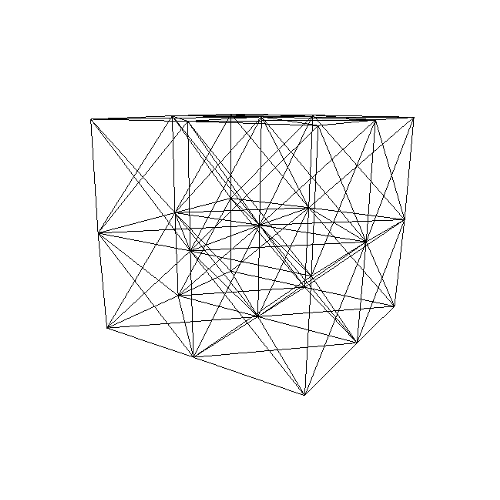
\includegraphics[width=7cm, height=7cm]{images/stabilny.png}
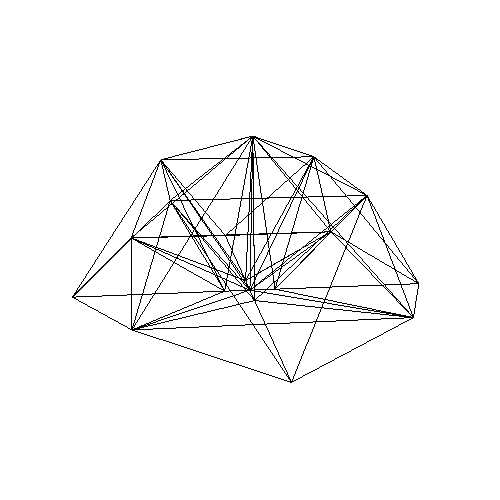
\includegraphics[width=7cm, height=7cm]{images/niestabilny.png}
\caption{Dwa stany stabilne dla sześciennego modelu.}
\label{stany}
\end{figure}

Rozwiązaniem problemu przechodzenia układu między stanami stabilnymi okazało się wprowadzenie sztucznej siły, pozwalającej zachować objętość. Takie podejście po raz pierwszy zaproponowano w \cite{rmofa}. Autorzy publikacji pogrupowali znajdujące się w układzie punkty masy w obiekty dla których można było zdefiniować objętość. Następnie w zależności od różnicy pomiędzy objętością spoczynkową a aktualną generowana była siła oddziałująca punkty masy. Kierunek tej siły jest zgodny z działaniem pewnej z góry zdefiniowanej normalnej. W \cite{isodb} autorzy przedstawiają bardziej ogólny przypadek przyjmując, że obiektem posiadającym objętość jest czworościan.Wierzchołki figury są punktami masy, a krawędzie sprężynami. Siła zachowawcza działająca na dany punktu masy $i$ czworościanu, określa się wzorem:

\begin{equation}
F_i^d = d_v ( v - v_0) n_i
\end{equation}
,gdzie $v$ jest aktualną objętością symulowanego czworościanu, $v_0$ jest jego spoczynkową objętością a $d_v$ jest arbitralnie zdefiniowaną stałą. $n_i$ jest to normalna przeciwległej ściany czworościanu. Podana metoda pozwala uniknąć odwrócenia wierzchołków symulowanego obiektu, ponieważ w takim przypadku obliczona objętość będzie ujemna i powstała, duża siła $F_i^d$ wymusi powrót układu do stanu wejściowego \cite{isodb}.

\subsubsection{Zależność od topologii}
W analizowanym modelu topologia połączeń między punktami mas jest z góry zdefiniowana. Można powiedzieć, że jest to kolejny parametrem symulacji, który w istotny sposób decyduje o jej jakości. Takie założenie samo w sobie nie jest błędne, gdyż modelując wewnętrzną strukturę ciała możemy określić jego fizyczną charakterystykę. Na przykład, symulując elastyczny sześcian i dodając dodatkowe połączenia między punktami masy w jednej płaszczyźnie otrzymamy obiekt różnie podatny na odkształcanie w zależności od kierunku działania siły. Taką mechaniczną właściwość ciała nazywany anizotropią. Anizotropia stanowi bardzo ciekawy przykład własności mechanicznej materiału, której implementacji w modelu punktów mas i sprężyn jest często problematyczna. 

Idealny model powinien umożliwiać symulowanie materiałów izotropowych (o własnościach mechanicznych niezależnych od kierunki działań siły) jak i anizotropowych. Poprzez możliwość manipulacji rozmieszczeniem punktów materialnych, sposoby ich połączeń sprężynami czy manipulowanie stałymi sprężystości, model dostarcza narzędzi do implementacji tych własności. Nie mniej jednak niektóre własności mogą pojawiać się wbrew wcześniejszym założeniom. Przykład niepożądanej anizotropii, otrzymanej poprzez różne struktury wewnętrzne modelu przedstawiono na rys. \ref{anizotropia}.

\begin{figure}[ht]
\centering
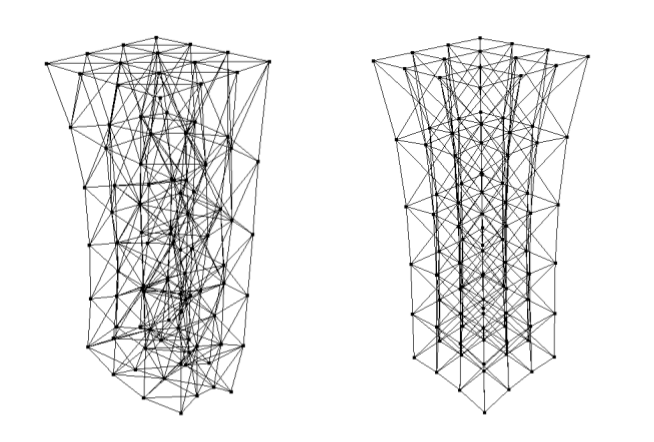
\includegraphics[scale=0.5]{images/anisotropy.png}
\caption{Porównanie dwóch zastosowanych siatek w obiekcie przytwierdzonym górną podstawą i poddanemu sile grawitacji. Lewo: Anizotropia obserwowana w czworościennej siatce połączeń. Prawo: Brak anizotropii w sześciennej siatce połączeń. Źródło: \cite{ca}}
\label{anizotropia}
\end{figure}

Okazuje się, że kalibracja parametrów modelu nie jest trywialna. W \cite{usa} autorzy proponuję metodę kalibracji poszczególnych stałych sprężystości sprężyn. Ich metoda pozwala na symulację zarówno izotropowych jak i anizotropowych. Jednak jak sami autorzy wskazują jest złożona obliczeniowo,a w publikacji została zaprezentowany tylko przykład dla siatek dwuwymiarowych. Inne podejście w swojej publikacji przedstawili francuscy badacze wykorzystując do estymacji parametrów sprężystości algorytmy genetyczne.\cite{ei}

Alternatywne podejście, odchodzące nieco od klasycznego modelu punktów mas i sprężyn, zostało przedstawione w publikacji D. Bourguignon i M-P. Cani \cite{ca}. Metoda ta, pochodna od systemu punktów mas i sprężyn, pozwala na definiowanie własności mechanicznych symulowanych obiektów niezależnie od przyjętej geometrii czy topologii. Pozwala to na wczytanie do symulacji obiektów utworzonych w programach do modelowania 3D i co ważniejsze, odciążenia grafika z konieczności uwzględnienia podczas pracy fizycznych charakterystyk modelu.\cite{ca}

Metoda zakłada, wszystkie punkty masy w modelu są pogrupowane w tzw. jednostki objętości (volume element), którymi najczęściej są czworościany. Dla każdej jednostki wyznacza się tymczasowe punkty masy położone wzdłuż stałych, predefiniowanych osi. Umiejscowienie osi ma odzwierciedlać mechaniczną charakterystykę obiektu. Z reguły stosuje się standardowo 3 osie, jednak możliwa jest też ich większa ilość \cite{ca}. Sposób wyznaczania punktów przecięcia przedstawiony jest na rysunku \ref{anizotropia-czworoscian}.

\begin{figure}[ht]
\centering
\begin{tikzpicture}

\coordinate (A) at (0, 0, 0);
\coordinate (B) at (6, 0, 0);
\coordinate (C) at (3, 0, 4.22);
\coordinate (D) at (3, 4.89, 2.11);

\draw[-] (D) -- (B) -- (C) -- (D) -- (A) -- (C);
\draw[-, dashed] (A) -- (B);

\filldraw[fill=red, draw=black] (A) circle (3pt);
\filldraw[fill=red, draw=black] (B) circle (3pt);
\filldraw[fill=red, draw=black] (C) circle (3pt);
\filldraw[fill=red, draw=black] (D) circle (3pt);

\node[above left] at (D) {A};
\node[below right] at (B) {B};
\node[below left] at (C) {C};
\node[below left] at (A) {D};

%intersection points
\coordinate (I1) at (barycentric cs:D=0.5,B=0.7,C=0.5);
\coordinate (I2) at (barycentric cs:A=0.7,B=0.5,D=0.5);
\coordinate (Imid) at (barycentric cs:I1=0.5,I2=0.5);

\filldraw[fill=blue, draw=black] (I1) circle (3pt);
\filldraw[fill=blue, draw=black] (I2) circle (3pt);
\node[above right] at (I1) {$P_1$};
\node[above left] at (I2) {$P_2$};
\node[below=25pt, right] at (I1) {$\alpha$};
\node[below=15pt, left] at (I2) {$\beta$};
\node[right, above=20pt] at (I1) {$\gamma$};

\draw[-,snake=snake] (I1) -- (I2);
\draw[<->,thick, shorten >=4pt, shorten <=4pt] (I1) -- (I2);
\draw[->,thick] (Imid) -- ++(0,0.6,0);
\draw[->,thick] (Imid) -- ++(0,-0.6,0);

\draw[-,densely dotted] (I1) -- (C);
\draw[-,densely dotted] (I1) -- (D);
\draw[-,densely dotted] (I1) -- (B);


\end{tikzpicture}

\caption{Wyznaczanie punktu przecięcia z osiami w czworościanie.}
\label{anizotropia-czworoscian}
\end{figure}

Przedstawiony czworościan posiada zdefiniowane dwie osie. Wyznaczono też dwa punkty przecięcia $P_1$ oraz $P_2$ z osią poziomą figury. W celu zapamiętania pozycji punktów przecięcia wyznacza się współczynniki kombinacji liniowej z wierzchołkami tworzącymi ścianę. $P_1 = \alpha * A + \beta *B + \gamma *C$. Współczynniki te muszą być wyznaczane dla czworościanu znajdującego się w stanie spoczynku. Punkty przecięcia traktowane są odtąd jak nowe punkty masy. Działają na nie siły wewnętrzne i zewnętrzne układu. Dwa punkty (zaznaczonymi na rys. \ref{anizotropia-czworoscian} kolorem niebieskim) zostają w istocie połączone sprężyną.

Następnie dokonuje się omawianych w poprzednich podrozdziałach obliczeń sił działających na punkt przecięcia. Mając dane współczynniki kombinacji liniowej, wyznaczyć można siły działające na punkty masy $A,B,C$ pierwotnie zdefiniowane w modelu. 

\begin{figure}[ht]
\centering
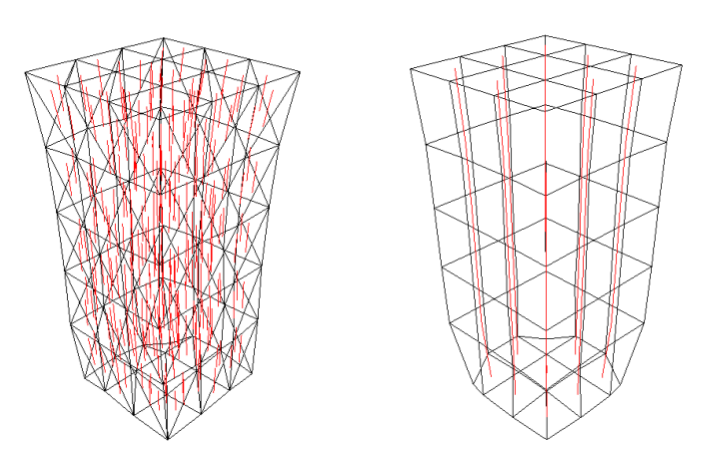
\includegraphics[scale=0.5]{images/fixed_anisotropy.png}
\caption{Porównanie dwóch zastosowanych siatek w obiekcie przytwierdzonym górną podstawą i poddanemu sile grawitacji. W modelu wykorzystano metodę D. Bourguignon i M-P. Cani, Źródło: \cite{ca}}
\label{anizotropia-czworoscian-fix}
\end{figure}

\subsection{Metody bazujące na pozycji}
